%%%%%%%%%%%%%%%%%%%%%%%%%%%%%%%%%%%%%%%%%%%%%%%%%
%-------------Préambule-------------------------%
%%%%%%%%%%%%%%%%%%%%%%%%%%%%%%%%%%%%%%%%%%%%%%%%%

\documentclass[12pt,a4paper,twoside]{report}
\usepackage[utf8]{inputenc}
\usepackage{amsmath}
\usepackage{hyperref} %pour table des matières
\usepackage{minitoc}
\usepackage[french]{babel}
\usepackage{array,multirow,makecell} %tableau
\newcolumntype{R}[1]{>{\raggedleft\arraybackslash }b{#1}}
\newcolumntype{L}[1]{>{\raggedright\arraybackslash }b{#1}}
\newcolumntype{C}[1]{>{\centering\arraybackslash }b{#1}}
\addto\captionsfrench{\renewcommand{\chaptername}{Partie}} %Changer nom de chapitre en partie
\usepackage[Glenn]{fncychap} %pour de super titres
\usepackage{glossaries} %pour le glossaire
\makeglossaries
\usepackage[left=2cm,right=2cm,top=2cm,bottom=2cm]{geometry} %Marge
\usepackage{amsfonts}
\usepackage{amssymb}
\usepackage{textcomp} %Pour les degres celsius
%\usepackage{xcolor} %pour les couleurs
\usepackage{amsmath,amsfonts,amssymb} %mathématiques
\usepackage{graphicx}
\usepackage{caption}
\usepackage{subcaption}
\usepackage{float}
\graphicspath{{./Images/}}
\usepackage{url}

%
%
% 

\newcommand{\Surtitre}{Rapport de BE}
\newcommand{\TitreRapport}{\textbf{Mesh and Computational Geometry}}
\newcommand{\DateStage}{Année scolaire 2019-2020}
\newcommand{\Annee}{2020}
\newcommand{\Eleve}{Colin CROS}
\newcommand{\Professeur}{Raphaëlle Chaine}
\newcommand{\Illustration}{illustration}
%
%
%

\renewcommand{\thesection}{\arabic{section}} %sections numérotées 1, 2...

\usepackage{listings}
\usepackage{color}
 
\definecolor{codegreen}{rgb}{0,0.6,0}
\definecolor{codegray}{rgb}{0.4,0.4,0.4}
\definecolor{codegraybis}{rgb}{0.6,0.6,0.6}
\definecolor{codepurple}{rgb}{0.58,0,0.82}
\definecolor{reddigits}{rgb}{0.64,0.08,0.25}
\definecolor{reddigits}{RGB}{169,17,1}
%\definecolor{backcolour}{RGB}{235,245,251}
%\definecolor{backcolour}{RGB}{253,250,254}
\definecolor{backcolour}{RGB}{250,244,254}
\definecolor{bluetitle}{RGB}{83,101,158}

\lstdefinestyle{mystyle}{
    backgroundcolor=\color{backcolour},   
    commentstyle=\color{codegraybis},
    keywordstyle=\color{blue},
    numberstyle=\color{codegray},
    stringstyle=\color{codegreen},
    basicstyle=\footnotesize,
    breakatwhitespace=false,         
    breaklines=true,                 
    captionpos=b,                    
    keepspaces=true,                 
    numbers=left,                    
    numbersep=5pt,                  
    showspaces=false,                
    showstringspaces=false,
    showtabs=false,                  
    tabsize=2,
    literate=
            {0}{{\textcolor{reddigits}{0}}}{1}
            {1}{{\textcolor{reddigits}{1}}}{1}
            {2}{{\textcolor{reddigits}{2}}}{1}
            {3}{{\textcolor{reddigits}{3}}}{1}
            {4}{{\textcolor{reddigits}{4}}}{1}
            {5}{{\textcolor{reddigits}{5}}}{1}
            {6}{{\textcolor{reddigits}{6}}}{1}
            {7}{{\textcolor{reddigits}{7}}}{1}
            {8}{{\textcolor{reddigits}{8}}}{1}
            {9}{{\textcolor{reddigits}{9}}}{1}
}
 
\lstset{style=mystyle}


\usepackage{fancyhdr} %pour un style de page personnalisé 
\pagestyle{fancy}

\renewcommand{\headrulewidth}{1pt}
\renewcommand{\footrulewidth}{1pt}
\fancyfoot[R]{\textbf{page \thepage}} 
\fancyfoot[C]{Colin CROS, École Centrale de Lyon}
\fancyfoot[L]{2019}
\fancyhead[LO]{\emph{\leftmark}}
\fancyhead[RO]{}
\fancyhead[RE]{\textit{\rightmark}}
\fancyhead[LE]{}

\begin{document}
\pagenumbering{arabic}
	

%%%%%%%%%%%%%%%%%%%%%%%%%%%%%%%%%%%%%%%%%%%%%%%%%%%%
%------------------Page de garde--------------------
%%%%%%%%%%%%%%%%%%%%%%%%%%%%%%%%%%%%%%%%%%%%%%%%%%%%

\thispagestyle{empty} %pour pas que ça numérote la page
\noindent %supprimer l'indentation


\begin{center}

	\begin{figure}[H]
	
\includegraphics[width=0.5\textwidth]{centrale_lyon}
	\end{figure}
	\vspace{5\baselineskip}
	
	\begin{center}
	{\Large \textbf{\Eleve}} \\ 
	\end{center}
	
	\vfill
	
	{\Large \textsc{\Surtitre}} \\
	\rule{9.5cm}{0.2pt} \\ %Trace trait horizontal
	\vspace{1\baselineskip} %espacement 
	{\LARGE \TitreRapport}
	\begin{figure}[H]
	\centering
	\includegraphics[width=0.8\textwidth]{\Illustration}
	\end{figure}

	
	\vfill
	\begin{table}[h!]
		\centering
		\begin{tabular}{r} %faire flotter tableau dans un environnement table colonne à 		gauche et à gauche
		\DateStage \\
		Professeur : \Professeur\\
		\end{tabular}
	\end{table}
			
\end{center}

\newpage

\newpage\section*{Introduction}

Ce rapport présente les différents rendus obtenus lors des BE du cours de Mesh and Computational Geometry. Les captures d'écran ont été réalisées sur les sorties du programme QT Creator implémenté pendant les BE (figure \ref{fig:programme}).

L'ensemble des codes du programme est disponible dans un répertoire github accessible à l'adresse : \url{https://github.com/TastyColin/Mesh-and-Computational-Geometry/}. Les fichiers des maillages utilisés (au format "off") sont également disponibles à cette adresse.

\begin{figure}[H]
	\centering
	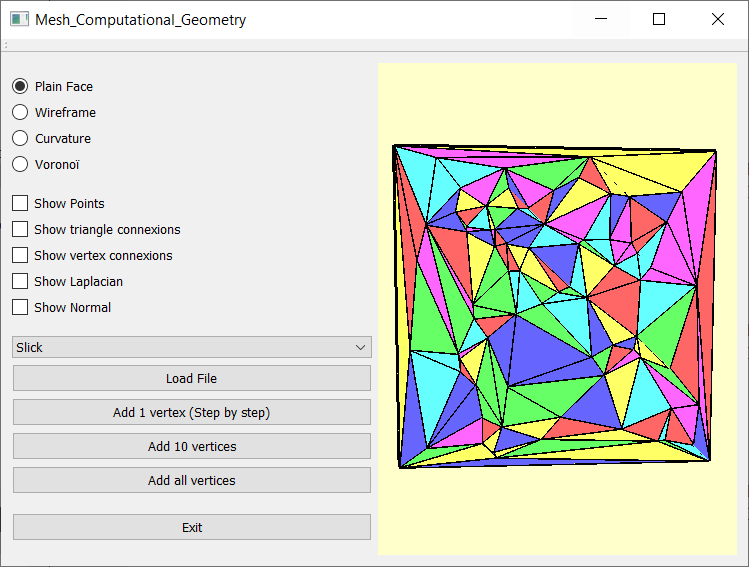
\includegraphics[scale=0.7]{programme.png}
	\caption{Programme réalisé pendant les BE.}
	\label{fig:programme}
\end{figure}

4 modes de visualisation sont disponibles dans le menu du programme qui affichent respectivement (de haut en bas) : les faces, les arêtes, la courbure et le diagramme de Voronoï associé à un fichier. Les "checkboxes" permettent d'ajouter des compléments d'information : les sommets, les différentes liaisons (triangle-triangle ou sommet-triangle), les normales, et le laplacien. Le menu déroulant sert à sélectionner un fichier que l'on importe grâce au bouton "Load File". Les 3 boutons d'ajout permettent de compléter la triangulation (uniquement sur le fichier "slick.off"). Une animation "pas à pas" a été implémentée lors de l'ajout d'un seul point pour illustrer les phases de recherche de point et de retournement des arêtes.

\newpage \section{Structure de données}

\subsection{Les fichiers OFF}
Les fichiers utilisés dans les BE étaient au format "off". Ce format de fichier est composé de trois types de lignes.
Tout d'abord, une ligne d'entête indiquant dans cet ordre le nombre de sommets, le nombre de faces et le nombre de trous. Viennent ensuite les lignes indiquant la position $x$, $y$, $z$ des sommets (une ligne par sommet). Et pour finir les lignes des faces qui débutent par le nombre de sommets constituant la face suivi de la liste des indices des sommets parcourues dans le sens trigonométrique (lorsque l'on regarde la face de l'extérieur).

Le séparateur utilisé est une espace. A titre d'exemple, voici le code réalisé pour un tétraèdre :
\begin{lstlisting}
4 4 0		# nb de sommets, nb de faces, nb de trous
0. 0. 0.	# sommet 1
1. 0. 0.	# sommet 2
0. 1. 0.	# sommet 3
0. 0. 1. 	# sommet 4
3 1 2 3		# face 1 (un triangle)
3 0 3 2 	# face 3 (un triangle)
3 0 1 3 	# face 2 (un triangle)
3 0 2 1 	# face 4 (un triangle)
\end{lstlisting}
Nous ne traiterons que des triangulations, en conséquence, toutes les faces seront triangulaires et sans trou.
\smallbreak
Trois fichiers "off" ont été réalisés : un tétraèdre, un cube et une pyramide à base carrée. Un quatrième fichier a été fourni, il s'agit d'un maillage du visage d'une femme. Les affichages de ces quatre maillages sont visibles sur la figure \ref{fig:plain_mesh}.

\begin{figure}[H]
	\centering
	\begin{subfigure}{.45\textwidth}
		\centering
		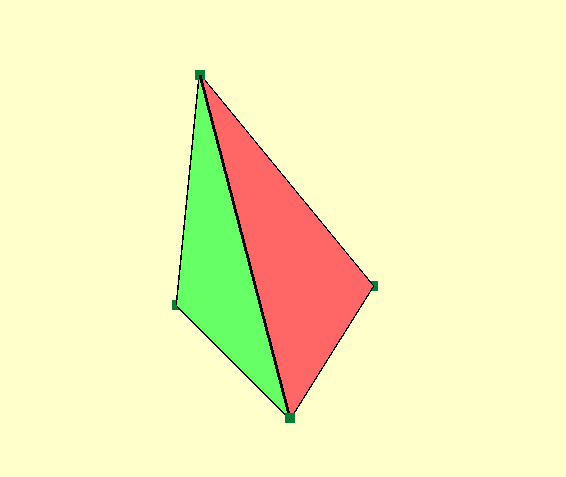
\includegraphics[width=\textwidth]{plain_tetraedre.png}
		\caption{Tétraèdre}
	\end{subfigure}
	\begin{subfigure}{.45\textwidth}
		\centering
		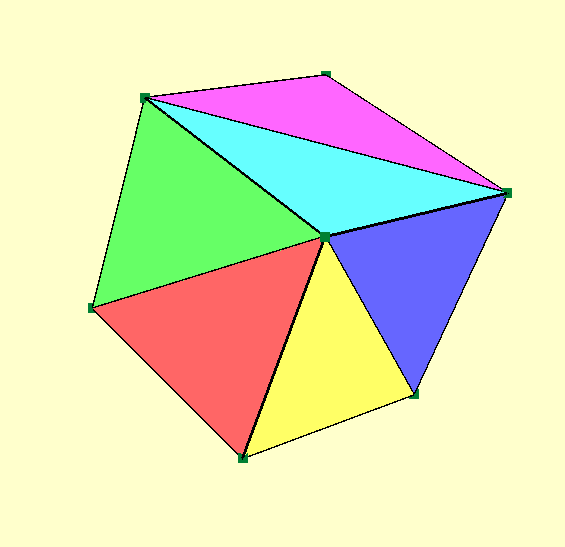
\includegraphics[width=\textwidth]{plain_cube.png}
		\caption{Cube}
	\end{subfigure}
	\begin{subfigure}{.45\textwidth}
		\centering
		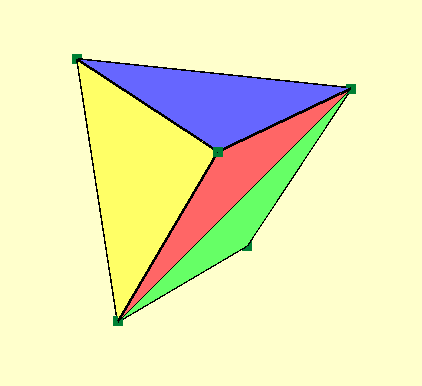
\includegraphics[width=\textwidth]{plain_pyramide.png}
		\caption{Pyramide à base carrée}
	\end{subfigure}
	\begin{subfigure}{.45\textwidth}
		\centering
		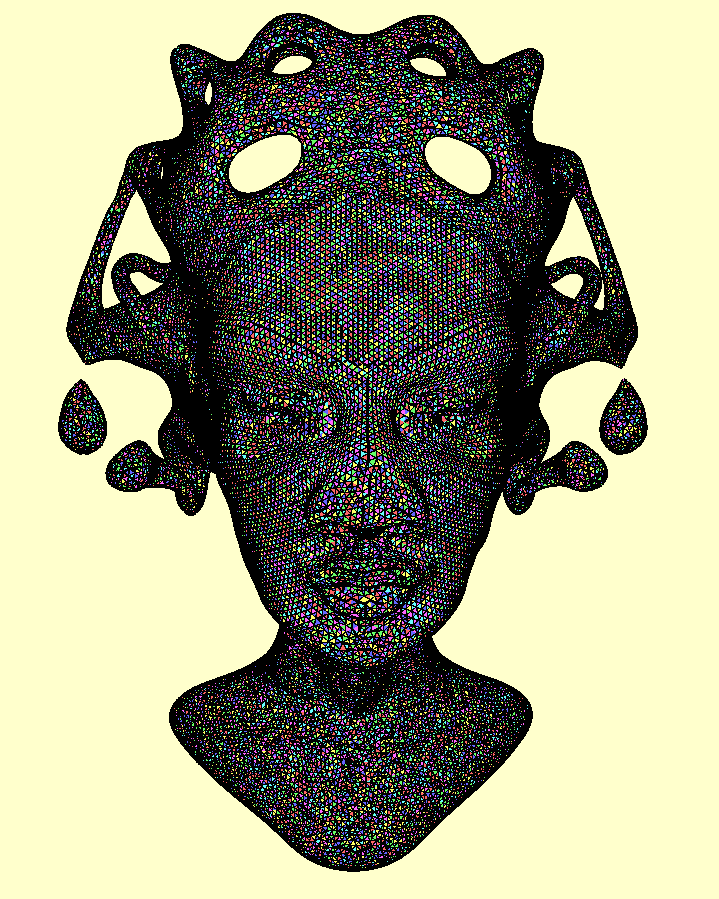
\includegraphics[width=\textwidth]{plain_queen.png}
		\caption{Visage}
	\end{subfigure}
	\caption{Différents maillages utilisés}
	\label{fig:plain_mesh}
\end{figure}

L'affichage est réalisé uniquement grâce aux positions des sommets des triangles. A ce stade, il est impossible de tourner autour d'un sommet ou de se déplacer de face en face. Les structures de données doivent être enrichies.

\subsection{Enrichissement des structures de données}

Deux structures principales composent les maillages : les sommets et les triangles. Les sommets comme les triangles seront stockés dans des vecteurs, on pourra donc les référencer grâce à leur indice.

\subsubsection{Les sommets}

Les sommets composent les faces des maillages. Un sommet est défini par un point, c'est-à-dire des coordonnées de l'espace, et l'indice d'un triangle qu'il compose. On enrichie la structure avec un second point qui servira à mémoriser le résultat de calculs ultérieurs, par exemple celui du laplacien.

\begin{lstlisting}
struct Vertex
{
    Point point;
    int i_triangle = -1;
    Point vector_value = Point(0,0,0);
};
\end{lstlisting}

\subsubsection{Les triangles}

Les triangles sont les éléments élémentaires des triangulations. Sans surprise, un triangle est défini par un triplet de sommets (on enregistrera leur indice), et un triplet d'indices de triangles correspondant à ceux des triangles adjacents.

\begin{lstlisting}
struct Triangle
{
	int i_vertices[3];
	int i_triangles[3];  
};
\end{lstlisting}

\smallbreak
Pour vérifier la bonne implémentation de ces deux structures de données, un segment représentant l'adjacence entre les triangles est affichage sur la figure. De même un segment reliant un sommet à sa face associé est affichable. La figure \ref{fig:liaisons} affiche ces deux types de liaisons.

\begin{figure}[H]
	\centering
	\begin{subfigure}{.4\textwidth}
		\centering
		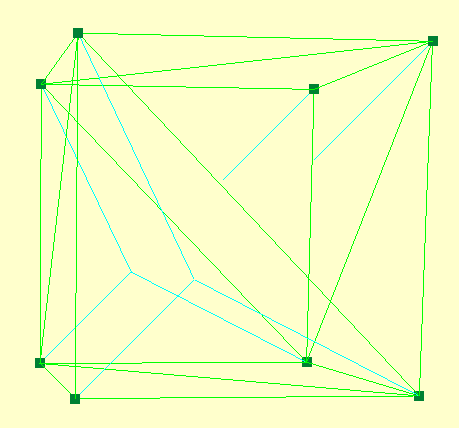
\includegraphics[width=\textwidth]{connexions_sommets_cube.png}
		\caption{Représentation des connexions entre un sommet et le centre de sa face associée sur un cube. Les segments relient les sommets au centre de leur face associée.}
	\end{subfigure}
	\begin{subfigure}{.4\textwidth}
		\centering
		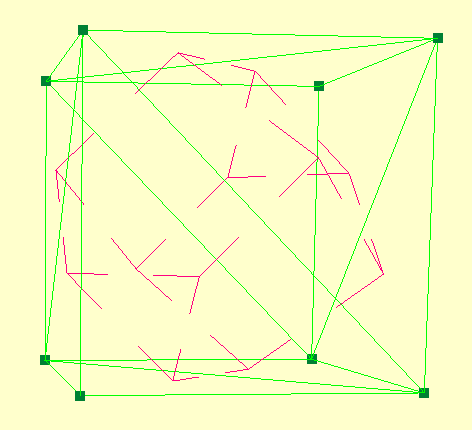
\includegraphics[width=\textwidth]{connexions_triangles_cube.png}
		\caption{Représentation des connexions entre les faces d'un cube. Les segments partent du centre d'un triangle et pointent vers le centre d'une face adjacente.}
	\end{subfigure}
	\caption{Représentation des différentes liaisons sur un cube}
	\label{fig:liaisons}
\end{figure}

\newpage\section{Circulateurs et calcul courbure}

Dans cette partie, nous allons réaliser le calcul et l'affichage de la courbure. Après avoir implémenté des circulateurs parcourant les faces ou les sommets incidents à un sommet donné. On peut calculer la normale et la courbure à ce sommet. On applique pour ce faire la formule faisant intervenir les cotangentes des angles adjacents qui a été donnée en cours et qui ne sera pas rappelée ici.

\begin{figure}[H]
	\centering
	\begin{subfigure}{.4\textwidth}
		\centering
		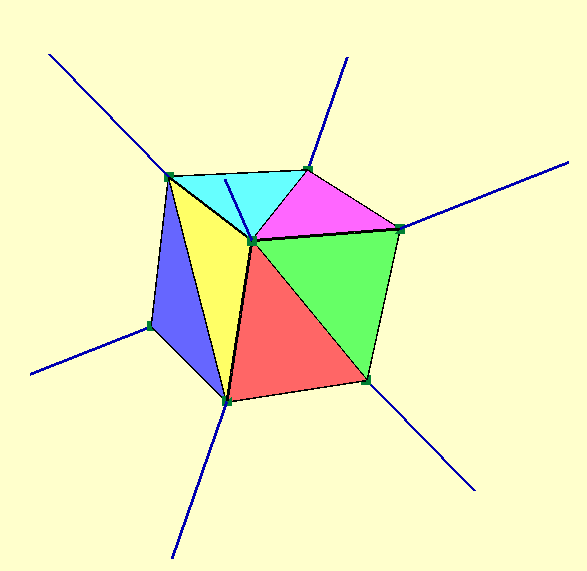
\includegraphics[width=\textwidth]{normales_cube.png}
		\caption{Affichage des normales du cube}			
		\label{fig:normales_cube}
	\end{subfigure}
	\begin{subfigure}{.4\textwidth}
		\centering
		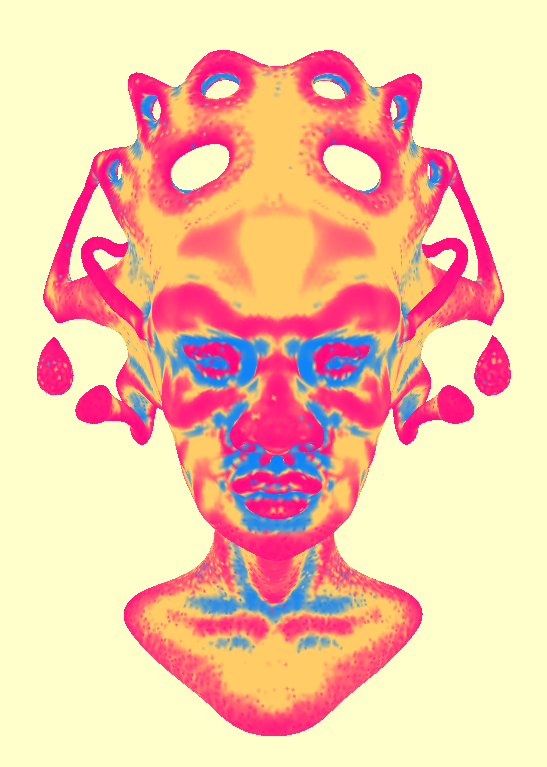
\includegraphics[width=\textwidth]{courbure_queen.png}
		\caption{Affichage des rayons de courbure sur le visage}					
		\label{fig:courbure_queen}
	\end{subfigure}
	\caption{Affichage de la courbure}
\end{figure}

Pour représenter les courbures, on affiche l'inverse du laplacien c'est à dire les rayons de courbure. La figure \ref{fig:courbure_queen} représente les rayons de courbure obtenus sur le maillage de visage. La plage de couleur a été choisie pour afficher en orangé les rayons de courbure grands en valeur absolue (ils correspondent aux zones plates), en rouge les petits rayons de courbures négatifs correspondant à des bosses (zones convexes) et en bleu les petits rayons de courbures positifs correspondant à des creux (des concavités).

\newpage\section{Triangulation de Delaunay et diagramme de Voronoï}

Afin de réaliser des triangulations Delaunay, un 5ème fichier "slick.off" a été ajouté (c.f. figure \ref{fig:slick}). Il contient une pyramide à base carrée avec 100 points tirés aléatoirement sur sa base. Ce fichier va permettre de réaliser les triangulations de Delaunay.

\begin{figure}[H]
	\centering
	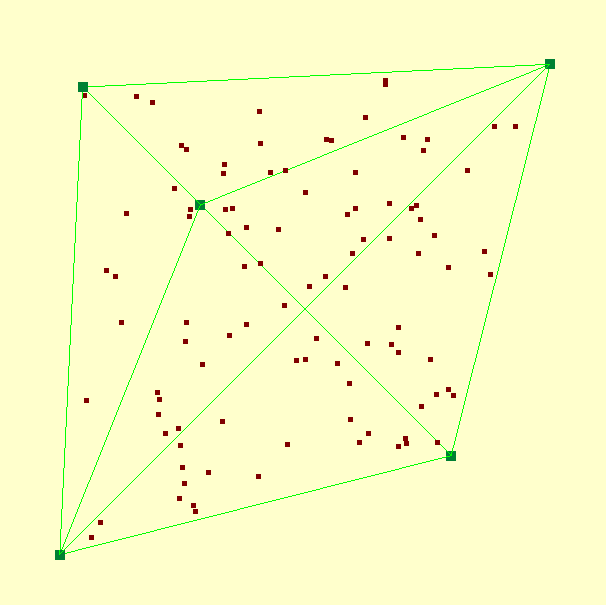
\includegraphics[scale=0.5]{slick.png}
	\caption{Visualisation du fichier "slick.off". Les points rouges ont été tirés aléatoirement et uniformément sur la base. Initialement, ils n'apparaissent dans aucun triangle.}
	\label{fig:slick}
\end{figure}

Pour réaliser la triangulation de Delaunay, les sommets sont ajoutés un à un au maillage en effectuant une marche par visibilité pour trouver le triangle dans lequel ils doivent être insérés. La figure \ref{fig:marche} illustre ce processus de recherche. Une fois le sommet inséré, pour maintenir le caractère global de Delaunay, une série de retournements d'arêtes est réalisée autour du nouveau sommet. Les triangles dont les arêtes sont testées lors de la phase de retournement sont illustrés figure \ref{fig:flip}.

\begin{figure}[H]
	\centering
	\begin{subfigure}{.4\textwidth}
		\centering
		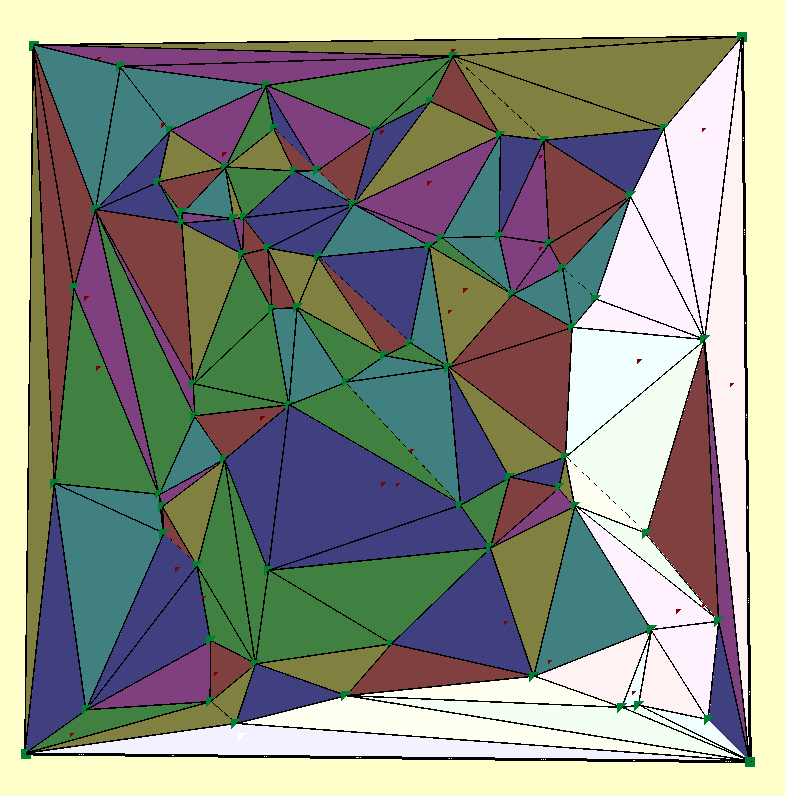
\includegraphics[width=\textwidth]{marche.png}
		\caption{Mis en lumière de la marche réalisé. Seuls les triangles clairs ont été testés (en commençant par le triangle le plus à droite).}			
		\label{fig:marche}
	\end{subfigure}
	\begin{subfigure}{.4\textwidth}
		\centering
		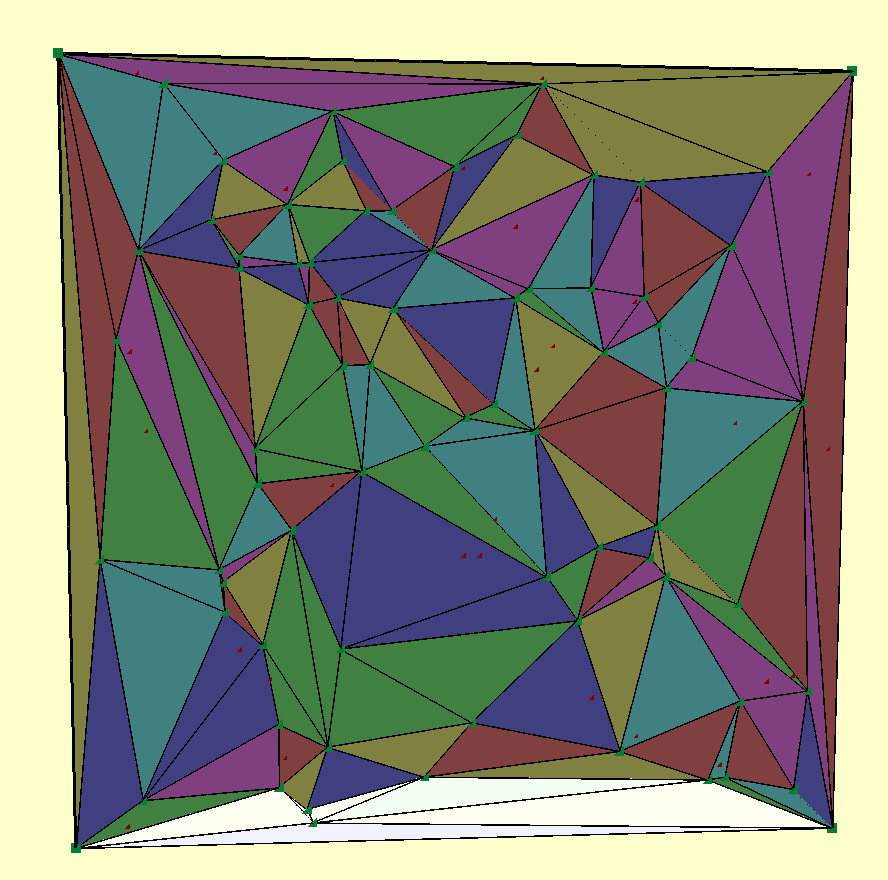
\includegraphics[width=\textwidth]{flip.png}
		\caption{Mis en lumière des triangles testés lors de l'étape de flip. L'animation est disponible dans le programme fourni.}					
		\label{fig:flip}
	\end{subfigure}
	\caption{Insertion d'un sommet}
\end{figure}

Enfin, à partir de la triangulation de Delaunay, on peut afficher le diagramme de Voronoï associé (figure \ref{fig:vornoi}). Pour cela on calcule et enregistre les coordonnées des centres des triangles qui sont nœuds du diagramme.

\begin{figure}[H]
	\centering
	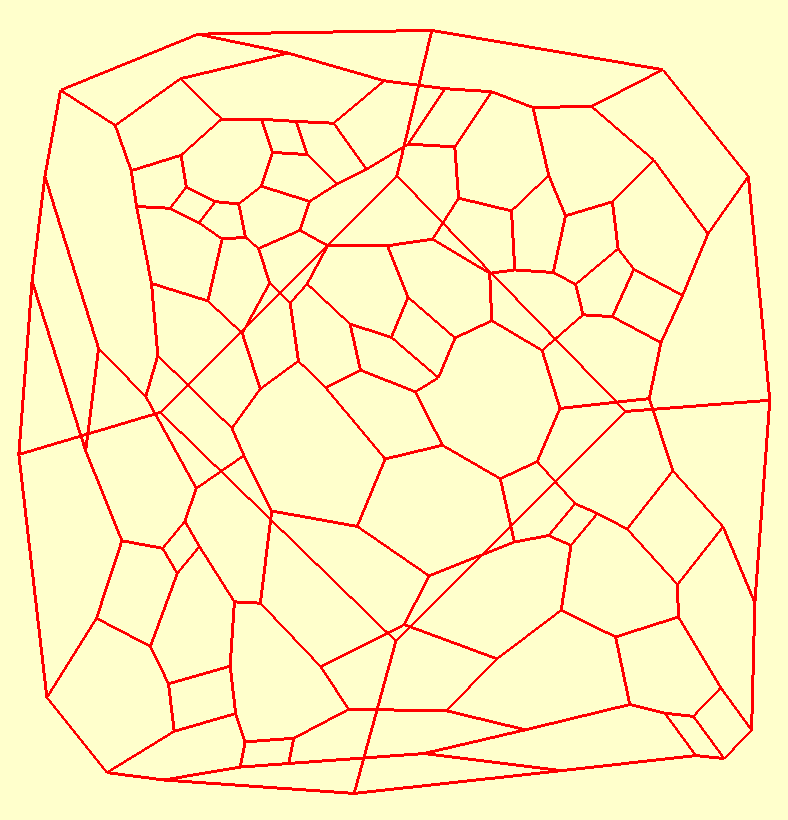
\includegraphics[scale=0.5]{voronoi.png}
	\caption{Diagramme de Voronoï associé à la triangulation précédente. Seul les arcs sont représentés, le losange du fond correspond aux faces de la pyramide.}
	\label{fig:vornoi}
\end{figure}

\newpage\section*{Conclusion}

Ces BE ont été l'occasion de comprendre les bases de l'informatique géométrique. En particulier de ce sensibilisé à ses subtilités, je pense notamment aux problèmes d'approximation que l'on néglige souvent mais qui peuvent s'avérer fatals pour certaines applications.

Je souhaiterais m'orienter vers les mathématiques appliquées à la navigation et je pense que les concepts étudiés durant ce MSO me seront utiles, à commencer par le simple fait d'avoir développé les programme en C++.

De manière générale, j'ai apprécié le format du cours : 2h de cours puis 2h de BE (un peu modulé en fonction des séances). Un léger point d'amélioration serait à mon sens le programme fourni au début des BE qui a l'air obsolète.  Par ailleurs, il faudrait aussi prévenir avant le premier cours d'installer QT Creator, pour ne pas souffrir de la connexion des salles de centrale.

\end{document}



